\section{RESULTS}
\label{sec:Res}

We evaluate our method on two widely used dataset: Hedau's dataset \cite{hedau2009recovering} and LSUN dataset \cite{zhang2015large}. 
\subsection{LSUN Results}
\label{sec:LSUN}
We train our multi-channel FCN on the relabeled LSUN dataset released by \cite{ren2016coarse}. The dataset consists of 4000 training, 394 validation, and 1000 testing images. We extract geometric hints from original images and resize all the images, depth and normal maps to $321\times321$ using bicubic interpolation. Then these three types of data are integrated to train the ResNet101 based multi-channel FCN. We evaluate our results using the official toolkit which provides two standard metrics: pixelwise error and corner error. The pixelwise error is computed by counting the percentage of pixels that are mismatched. (The Hungarian algorithm is applied to address the labeling ambiguity problem) The corner error is computed by calculating the Euclidean distance between predicted corners and corresponding ground truth corners.

Our performance on LSUN test set compared with other methods is shown in Table~\ref{table:comparison-lsun}. While Zhao et al.~\cite{zhao2017physics} train their FCN on SUNRGBD dataset, we do not use external data. Fig.~\ref{fig:qualitative} display some qualitative results of our method. 

\begin{figure}[!ht]
	\centering
	\textsc{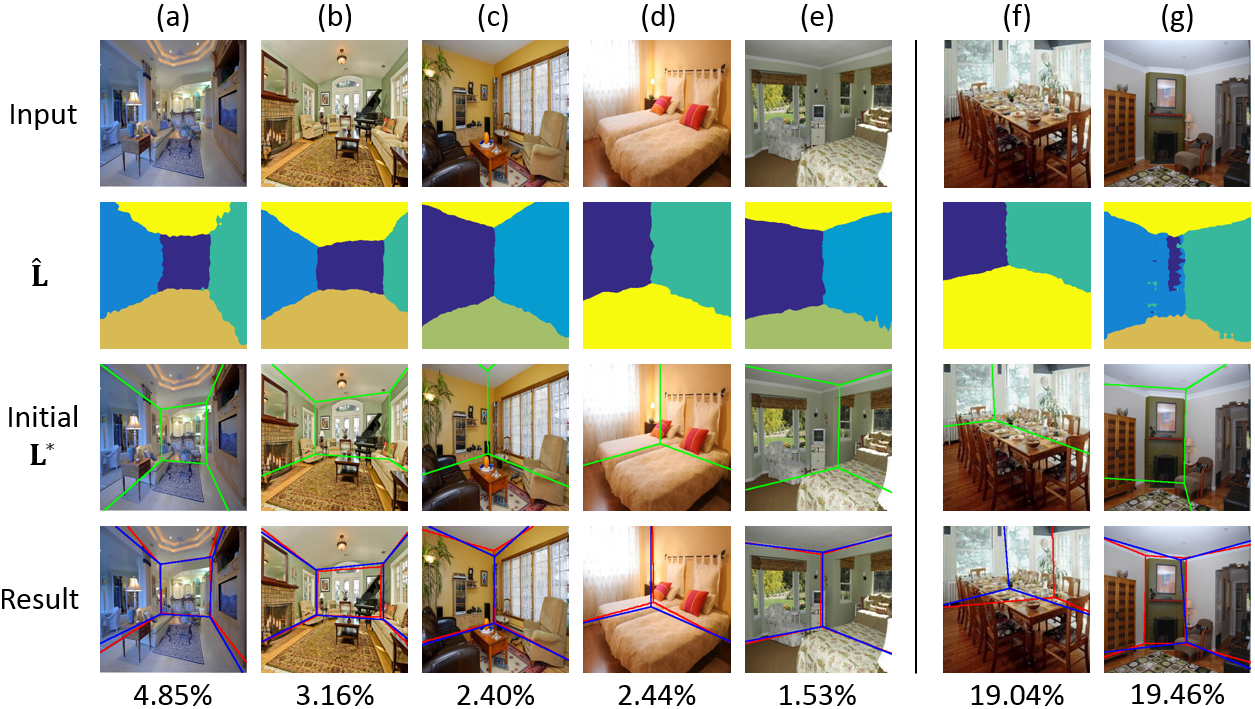
\includegraphics[width=8.5cm]{figure/qualitive.png}}
	\caption{Qualitative results on LSUN validation set. (a)-(e) depict precise results. (f)(g) show failure cases misled by $\vb{\hat{L}}$. }
	\label{fig:qualitative}
\end{figure}

\begin{table}
	\centering 
	\begin{tabular}{l|c|c}
		\hline 
		Method & Corner Error (\%) & Pixel Error (\%) \\
		\hline
		Hedau et al. (2009)~\cite{hedau2009recovering} & 15.48 & 24.23 \\
		Mallya et al. (2015)~\cite{mallya2015learning} & 11.02 & 16.71 \\
		Zhang et al. (2017)~\cite{zhang2017learning} & 8.70(5.17) & 12.49(6.58) \\
		Dasgupta et al. (2016)~\cite{dasgupta2016delay} & 8.20 & 10.63 \\
		Ren et al. (2016)~\cite{ren2016three} & 7.95(5.23) & 9.31(7.57) \\
		Zhao et al. (2017)~\cite{zhao2017physics} & 3.84 & 5.29 \\
		Proposed MC-FCN & 6.26 & 8.61 \\
		\hline
	\end{tabular}
	\caption{Performance on the LSUN~\cite{zhang2015large} dataset}	
	\label{table:comparison-lsun}
\end{table}

\subsection{Hedau Results}
\label{sec:Hedau}
We also conduct experiment on a relatively smaller dataset published by \cite{hedau2009recovering}, which consists of 209 training images and 104 testing images. We directly predict the semantic surface on Hedau's test set using the model trained on LSUN. Pixel error is adopted to evaluate the results, see Table~\ref{table:comparison-hedau}. Our performance is better than \cite{ren2016three} which has finetuned their model on Hedau's training set. This indicates that our model has a good generalization ability.

\begin{table}
	\centering 
	\begin{tabular}{l|c}
		\hline 
		Method & Pixel Error (\%) \\
		\hline
		Hedau et al. (2009)~\cite{hedau2009recovering} & 21.20 \\
		Mallya et al. (2015)~\cite{mallya2015learning} & 12.83 \\
		Zhang et al. (2017)~\cite{zhang2017learning} & 12.7 \\
		Dasgupta et al. (2016)~\cite{dasgupta2016delay} & 9.73 \\
		Ren et al. (2016)~\cite{ren2016coarse} & 8.67 \\
		Zhao et al. (2017)~\cite{zhao2017physics} & 6.60 \\
		Proposed MC-FCN & 8.49 \\
		\hline
	\end{tabular}
	\caption{Performance on the Hedau's~\cite{hedau2009recovering} dataset}
	\label{table:comparison-hedau}
\end{table}


\subsection{Analysis of Geometric Hints}
\label{sec:ablation}
To explore the benefits of geometric hints for semantic surface segmentation, we train FCNs with or without geometric information as additional input. Their performance are evaluated on LSUN validation set using pixel accuracy of $\vb{\hat{L}}$. To compare with \cite{ren2016coarse, dasgupta2016delay}, both of which are built on VGG16, we train our MC-FCN based on VGG16 too. For \cite{ren2016coarse}, we directly apply their trained model to generate $\vb{\hat{L}}$. And for \cite{dasgupta2016delay}, we train an FCN having the same architecture in \cite{dasgupta2016delay}. Qualitative results are demonstrated in Fig.~\ref{fig:fcn-comparison}. Intuitively, the geometric hints help remove the spurious regions caused by clutter and generate more accurate semantic segmentation. Quantitive results are shown in Table~\ref{table:ablation}. We also train a classic FCN-32s without incorporating geometric hints for comparison.

\begin{figure}[!ht]
	\centering 
	\textsc{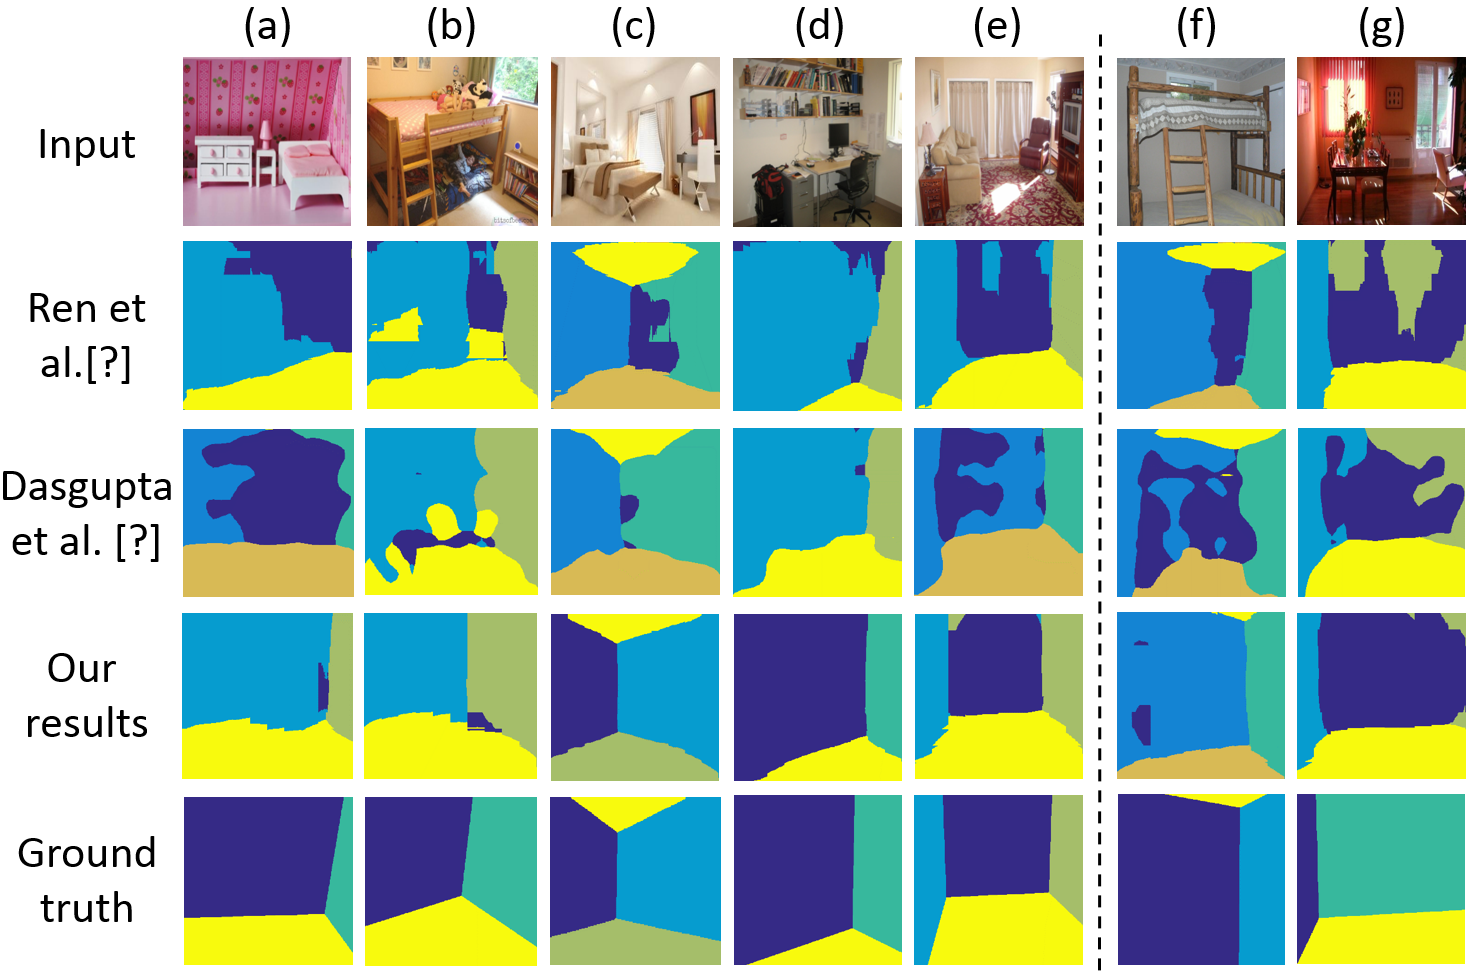
\includegraphics[width=8.5cm]{figure/compare.png}}
	\caption{Surface segmentation results using different architectures. All the networks are built on VGG16 architecture. Our MC-FCN with geometric hints generates more robust segmentation facing complex environmental factors.}
	\label{fig:fcn-comparison}
\end{figure}

\begin{table}
	\centering
	\begin{tabular}{c|c}
		\hline
		Network & Pixel Accuracy\\
		\hline
		Ren et al.~\cite{ren2016coarse} & 78.46 \\
		FCN-32s & 81.09 \\ 
		Dasgupta et al.~\cite{dasgupta2016delay} & 84.14 \\ 
		Proposed MC-FCN  & 85.95 \\
		\hline
	\end{tabular}
	\caption{Pixel accuracy of semantic surface segmentation by different FCNs. By utilizing geometric hints, our proposed MC-FCN acquire more accurate segmentation. }	
	\label{table:ablation}
\end{table}

